\subsection{Temperatur}\label{subsec:Temperatur}
Um einen Einblick in das Temperaturverhalten des Motors zu erlangen, wurde in diesem Versuch die Erwärmung in Abhängigkeit der Drehzahl bei konstantem Moment gemessen. Die Messung erfolgte bei einer Drehzahl von 1550 RPM und bei 2550 RPM, und einem jeweiligen Drehmoment von 32Nm. Die Starttemperatur des Motors lag jeweils bei ca. 60°C und wurde solang betrieben, bis er eine Betriebstemperatur von 100°C erreicht hatte. Der Versuch in der Abbildung \ref{fig:Temperatur} wurde ohne zusätzliche Ventilation des Motors durchgeführt. Alle Versuche wurden unter den Bedingungen \ref{tab:Temperatur} durchgeführt.



\begin{table}[H]
	\centering
	\begin{tabular}{C{4cm} C{4cm} C{3cm}} 
		\multicolumn{3}{c}{\textbf{Versuchsbedingungen}} \\
		{Messgrösse}& {Bedingung} & {Wert}\\ \hline\hline 
		Spannung (DC)   & konstant &   96 V     \\
		Strom (DC)   & vernachlässigt &   -     \\
		Leistung (AC)   & vernachlässigt &   -    \\
		Drehzahl   & konstant &   1500/2500 RPM    \\
		Drehmoment-Sollwert   & konstant &   32 Nm    \\
		Motor-Temperatur   & gemessen &   40-100 °C    \\
		Controller-Temperatur   & gemessen &   35-64 °C    \\
	\end{tabular}
	\caption{Versuchsbedingungen Temperatur}\label{tab:Temperatur}
\end{table}

\begin{figure}[H]
	\centering
	\includegraphics[width=0.8\linewidth]{Temperatur.jpg}
	\caption{Erwärmung}\label{fig:Temperatur}
\end{figure}


Da die Leistung sowohl vom Drehmoment als auch von der Drehzahl abhängig ist, wurde  der Motor beim Versuch mit 2550RPM mit einer höheren Leistung betrieben, womit auch ein grössere Strom fliesst. Aus diesem Grund ist die Erwärmung des Motors bei höheren Drehzahlen dementsprechend grösser. In der Abbildung \ref{fig:TemperaturMotor} und \ref{fig:TemperaturController} sind der Temperaturverlauf des Motors und des Controllers ersichtlich. Beim Motor wurde zuerst die Messung mit nur einem zusätzlichen Ventilator gemessen und anschliessend mit drei zusätzlichen Ventilatoren. Beim Controller wurde die Messung zuerst mit einem grossen thermischen Kühlkörper (der Messtisch diente als Kühlkörper) und zum anderen ohne Kühlkörper (thermische Isolation zum Messtisch) durchgeführt. Bei diesen Versuche wurde auch die Zeit zum Abkühlen gemessen. Diese Versuche wurden jeweils mit einer Drehzahl von 2500 RPM durchgeführt.


\begin{figure}[H]
	\centering
	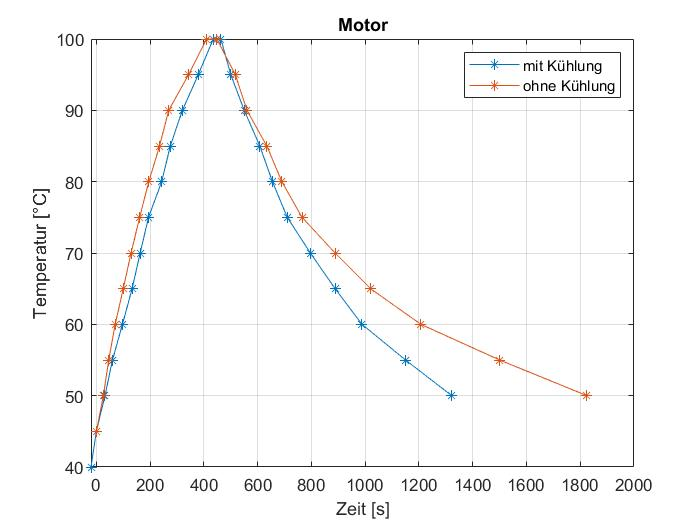
\includegraphics[width=0.8\linewidth]{TemperaturMotor.jpg}
	\caption{Temperaturverlauf Motor}\label{fig:TemperaturMotor}
\end{figure}

In der Temperaturkurve des Motors ist ersichtlich, dass die Zeit zum Abkühlen bedeutend grösser ist als welche der Erwärmung bei Nennmoment. Das der Motor im Abrollbetrieb mit einem hohen Wiederholungsintervall (VERWEIS AUF ANDERES KAPITEL) betrieben werden kann, muss der Motor zusätzlich gekühlt werden.

\begin{figure}[H]
	\centering
	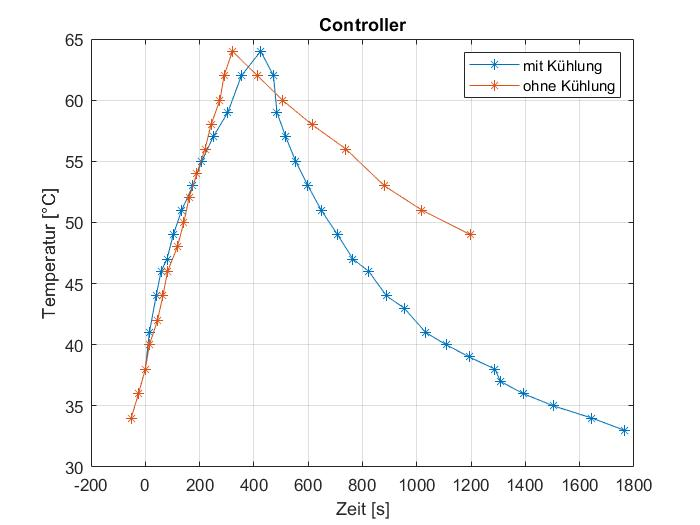
\includegraphics[width=0.8\linewidth]{TemperaturController.jpg}
	\caption{Temperaturverlauf Controller}\label{fig:TemperaturController}
\end{figure}

Bei diesem Versuch ist ersichtlich, dass der Controller ohne Kühlung viel langsamer abkühlt. Der Hersteller weisst im Datenblatt jedoch keine max. Temperatur aus (VERWEIS AUF DATENBLATT), weswegen wir eine Temperaturgrenze von 65°C annehmen.